\documentclass [11pt]{article}
\usepackage[a4paper, margin=1in]{geometry}

\usepackage[british]{datetime2}

\usepackage[hidelinks]{hyperref}
\usepackage{amsmath}
\usepackage{subfig}
\usepackage{graphicx}
\graphicspath{{graphics/}}
\usepackage{float}
\usepackage{cleveref}
%\usepackage{minted}
%\setminted[r]{fontfamily=courier}

\usepackage[T1]{fontenc}
\usepackage{lmodern}
\usepackage{titlesec}

\usepackage{algorithm}
\usepackage{algpseudocode} 

\usepackage{booktabs}

\usepackage[backend=biber, bibencoding=utf8, sorting=none]{biblatex}
\addbibresource{references.bib}

\usepackage{listings}
\lstset{basicstyle=\ttfamily}
%\newcommand{\cmd}[1] {\lstinline[breaklines=true]|git -> #1|}
\newcommand{\cmd}[1] {\lstinline[breaklines=true]|#1|}

\titleformat{\section}{\normalfont\Large\bfseries}{Assignment \thesection:}{1em}{}


\begin{document}
\begin{titlepage}
		\centering
		\includegraphics[scale = 0.4]{logo.pdf}\\[0.5 cm]
		\textsc{\LARGE politecnico di torino}\\[4 cm]

				
		\rule{\linewidth}{0.2 mm} 
		{ \huge Complex networks: theory and applications\\Laboratory report}
		\rule{\linewidth}{0.2 mm} \\[4.5 cm]

			\LARGE Andrea Senacheribbe\\s265392\\[4cm]
		\Large Master in Communications and Computer Networks Engineering\\[0.7cm]

		
		\Large 4th July 2019	
		
\end{titlepage}

\newgeometry{top=1.5in,bottom=1.5in,right=1in,left=1in}
\section{Centrality indices}
%!TeX root = ../complex_net_report_senacheribbe.tex
\graphicspath{{../assignment1/figures/}}

\subsection{Introduction}

In this first assignment, we evaluate the centrality of the nodes in a medium size graph (some thousands of nodes), using different centralities measures.\\
The graph chosen for the following analysis is a protein-protein interaction (PPI) graph in Homo Sapiens (taken from \cite{db_react}). The nodes represents proteins and two nodes are connected by an edge if they have some kind of interaction.\\
The centralities in protein-protein interaction networks are a powerful tool to understand which proteins play an important role and are essential for the organism.

\subsection{Graph properties}
First of all, the graph is read from file and processed to remove self-loops and extract only the largest connected component.
The resulting graph has  $n = 5973$ vertices and $m = 145778$ edges. It is stored by employing its adjacency matrix represented in sparse matrix format.
The structure of the matrix is shown in the sparsity plot of \cref{fig:1_sparsity}.

\begin{figure} [!ht]
	\centering
	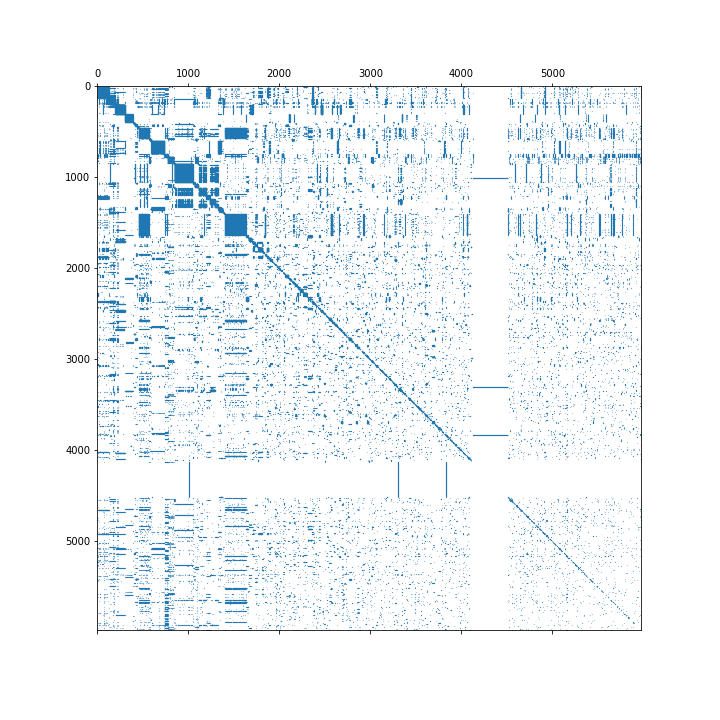
\includegraphics[width=.5\linewidth, clip, trim={2cm 2cm 2cm 2cm}]{sparsity}
	\caption{Sparsity of PPI graph with  $n = 5973$ and $m = 145778$}
	\label{fig:1_sparsity}
\end{figure}
For completeness we also report in  \cref{fig:1_surv_log} the degree distribution through the survival function (inverse cumulative) in log log scale. We can notice that the distribution doesn't follow a powerlaw, since its plot has not a linear behaviour in the log log plot.

\begin{figure} [!ht]
	\centering
	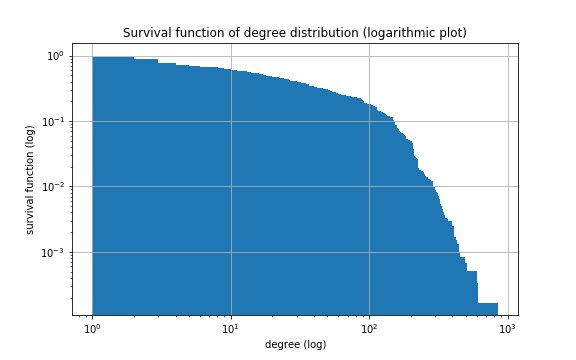
\includegraphics[width=.5\linewidth]{deg_distr_surv_log}
	\caption{Survival function of degree distribution}
	\label{fig:1_surv_log}
\end{figure}
\pagebreak

\subsection{Degree centrality}

The first and easier centrality index studied is the degree centrality. It is defined for node $i$ as
\begin{equation}
C_{deg}(i)=\frac{deg(i)}{\max_{j}  deg(j) }
\end{equation}
where $deg(i)$ is the degree of node $i$.\\
The measure is normalized dividing by the maximum degree, so that $0\leq C_{deg} \leq 1$.
The value of $C_{deg}$ for each node is depicted in \cref{fig:1_deg_centrality}.

\begin{figure} [!ht]
	\centering
	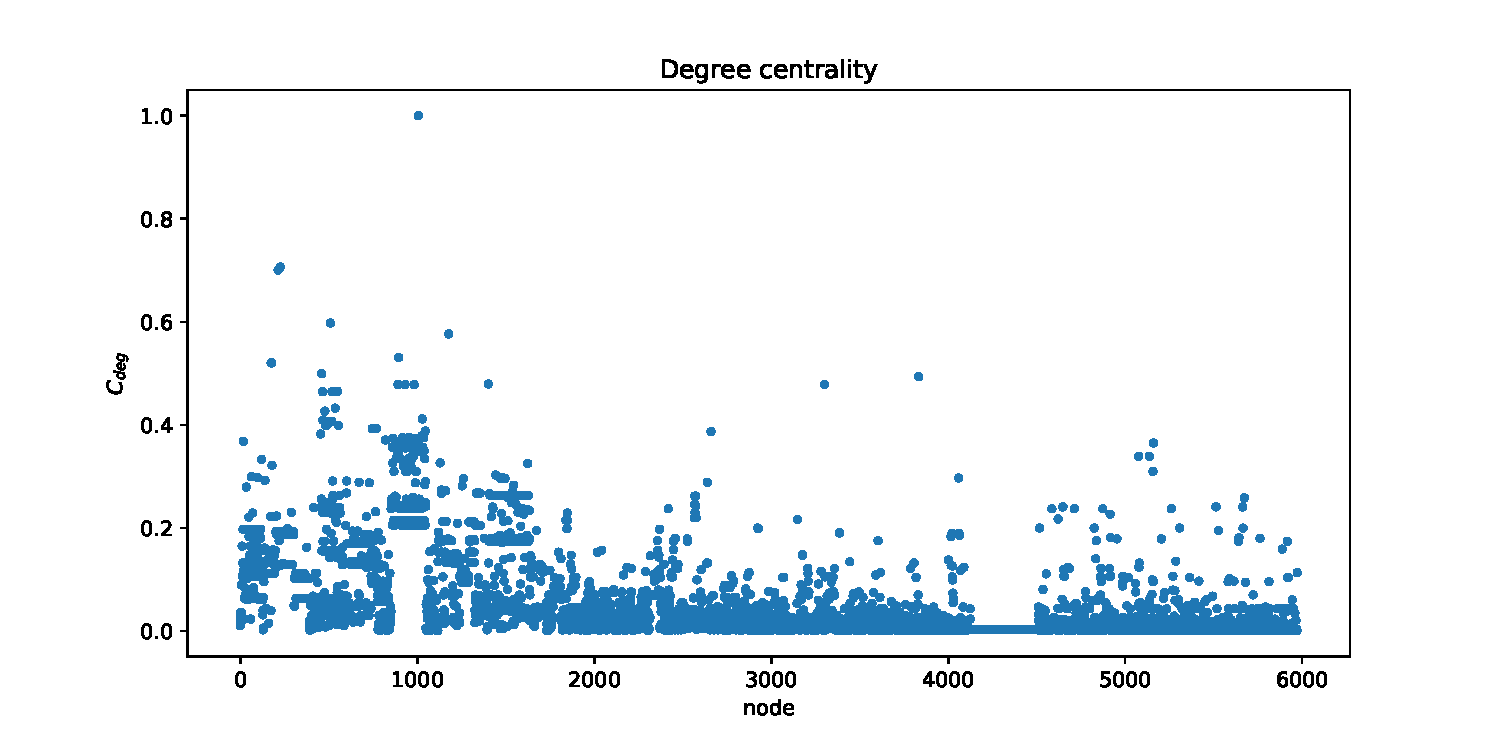
\includegraphics[width=.55\linewidth]{deg_centrality}
	\caption{Value of degree centrality for each node in the graph}
	\label{fig:1_deg_centrality}
\end{figure}

Even if very simple to compute, the degree centrality can give us useful indications of which node is more important in the network. Its limitation is that it only counts the number of adjacent nodes and doesn't exploit the structure of the graph.


\subsection{Katz centrality}
Katz centrality tries to assign an importance to each vertex according to the importance of its neighbours. This is an iterative process that at the end should converge to a final solution, which is the resulting centrality for every node. 
For a vertex $i$ in the graph, the Katz centrality is defined as
\begin{equation}\label{eq:1_katz}
x_i=\alpha \sum_{j}{A_{ij}x_{j}} + \beta_i
\end{equation}
where $A_{ij}$ is the adjacency matrix of the graph and $\beta_i=1$ to give an initial importance to all vertices.

To guarantee convergence the factor $\alpha$ is chosen such that $\alpha<1/\lambda_1$ with $\lambda_1$ largest eigenvalue of $A$.
For our network, $1/\lambda_1 \approx 0.004807$ and so we chose $\alpha=0.002$. $\lambda_1$ was calculated using numerical methods on sparse matrix.

The above \cref{eq:1_katz} can also be expressed in matrix form
\begin{equation}\label{eq:1_katz_mat}
\mathbf{x}=\alpha \mathbf{A} \mathbf{x} + \mathbf{1} \implies (\mathbf{I} - \alpha  \mathbf{A}) \mathbf{x}= \mathbf{1}
\end{equation}
and solved for $\mathbf{x}$ using specific solvers for sparse matrices, without expanding $\mathbf{A}$ to dense format.

The Katz centrality $C_{ka}$ (above was indicated as $\mathbf{x}$ for brevity) is calculated in both ways: with 1000 iterations of \cref{eq:1_katz} and by solving the system in \cref{eq:1_katz_mat}. With both methods, we obtained the same result up to approximation errors ($\approx 10^{-15}$). Fig. \ref{fig:1_katz_centrality} shows the value of $C_{ka}$ for each node.

\begin{figure} [!ht]
	\centering
	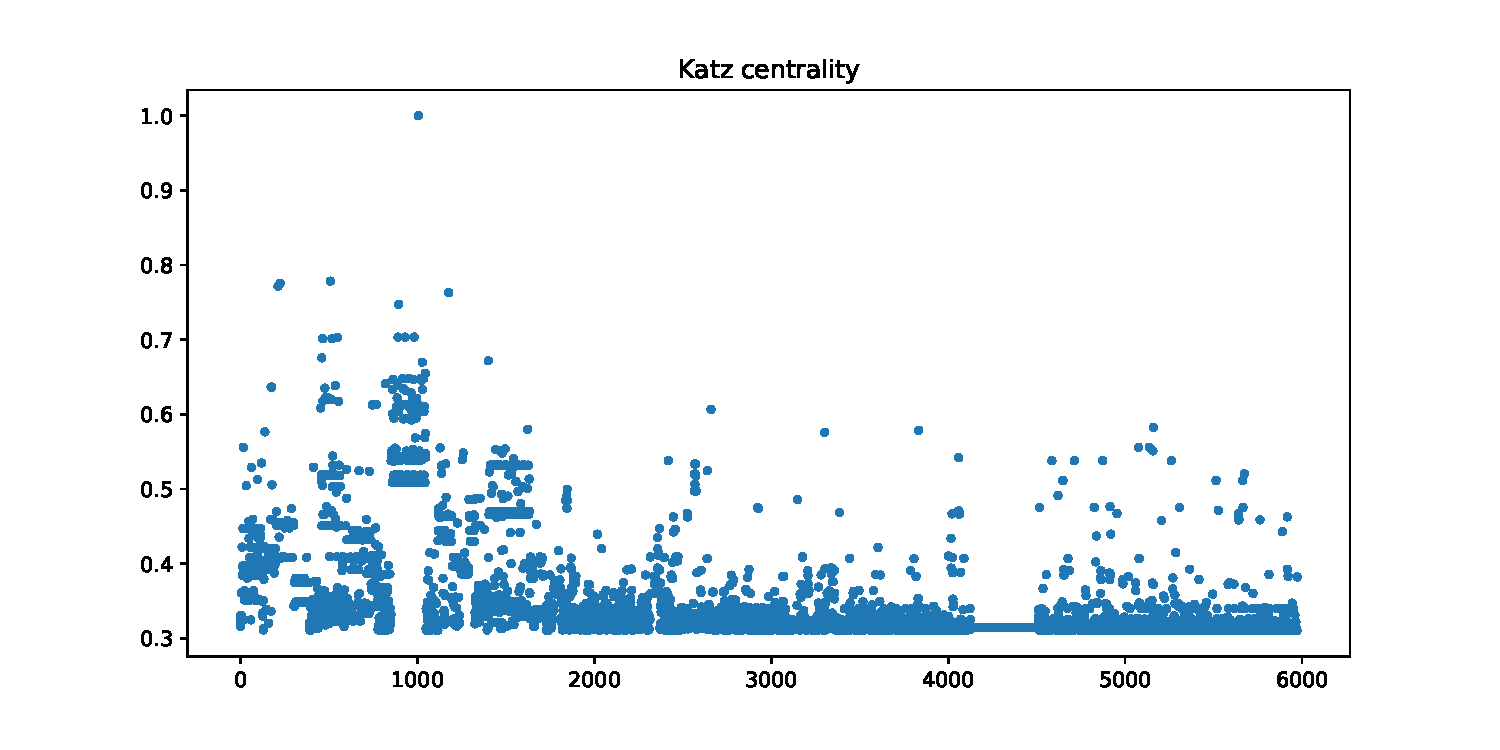
\includegraphics[width=.55\linewidth]{katz}
	\caption{Value of Katz centrality for each node in the graph}
	\label{fig:1_katz_centrality}
\end{figure}


\subsection{Betweenness centrality}

The last centrality considered is the betweenness centrality. It evaluates the importance of a node $i$ according to how many shortest paths pass through it. In particular,
\begin{equation}\label{eq:1_betw}
C_{betw}(i)= \sum_{s,t \neq i}{\frac{\sigma_i(s,t)}{\sigma(s,t)}}
\end{equation}
where $\sigma_i(s,t)$ is the number of shortest path from $s$ to $t$ passing through $i$ and  $\sigma(s,t)$ is the total number of shortest path from $s$ to $t$.\\
Notice that in case of parallel shortest paths, their effect on the centrality is split equally among them (we divide by their number $\sigma(s,t)$).

A simple algorithm to calculate betweenness centrality can be to compute all the shortest paths between any couple of nodes $(s,t)$ and count how many times these paths pass through node $i$, weighting by the number of shortest path from $s$ to $t$. This algorithm runs in $O(n^3)$, which can be too much for large networks.\\
A better solution for sparse graphs (as our case) is the Brandes' algorithm which runs in $O(n m)$. The basic idea is to perform an augmented BFS that keeps also the count of how many shortest paths are found. The graph is visited then in the reverse order to aggregate the results. A more detailed explanation of the algorithm is given in \cite{brandes_slides}, while the pseudocode, which we implemented in actual code, is available in the original paper \cite{brandes}.
In \cref{fig:1_between} the result of the algorithm on our graph is reported. The values are normalized so that $C_{betw} \in [0,1]$.

\begin{figure} [!ht]
	\centering
	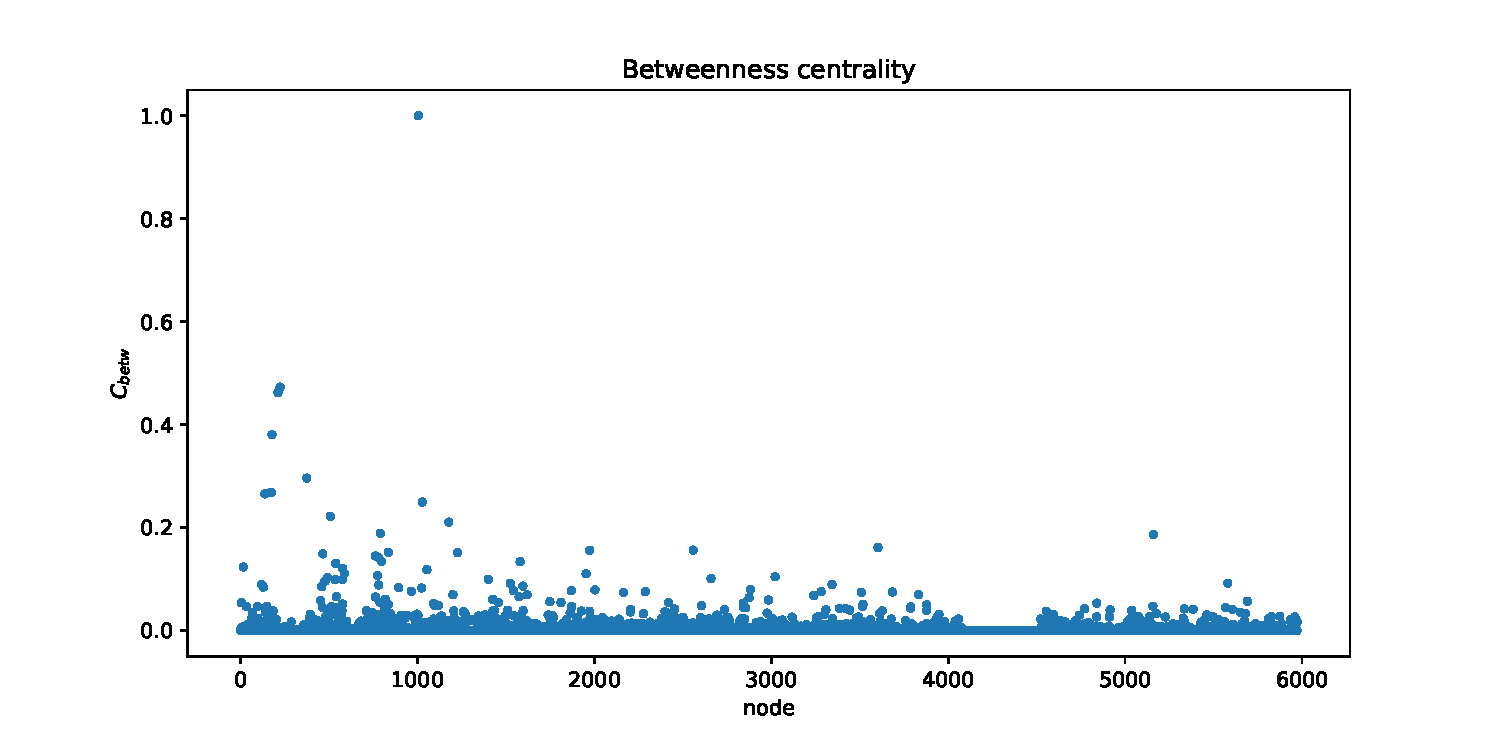
\includegraphics[width=.55\linewidth]{betweenness}
	\caption{Value of betweenness centrality for each node in the graph}
	\label{fig:1_between}
\end{figure}

\subsection{Final comparison and conclusions}
We can now draw a comparison among the different metrics considered. Degree, Katz and betweenness centralities for each node are plotted in \cref{fig:1_comparison_n}. Instead in \cref{fig:1_comparison_sort}, they are represented all sorted according to increasing Katz centrality.\\
We can notice that degree and Katz centrality are correlated and both follow the same trend. Betweenness centrality instead produces low values for most of the nodes (see also \cref{fig:1_between}), and peaks only for some of them, which are the central nodes in the networks where most of the paths pass. The different trend is due to the completely different way to compute the metric: betweenness looks for shortest paths in the whole network, while the others looks only to the adjacent nodes.
\\Interestingly, all the centralities assume value $1$ (maximum) for node $\#1006$. Therefore they all agree this is the most important node in the graph. 

In our case of protein-protein interaction graph, this indicates that $\#1006$ is the most important protein, which can be the focus to further studies and analyses by domain experts. But this result was obtained only by looking to the mathematical structure of the graph, without any labelling or knowledge about what the nodes represent. This proves the effectiveness of these methods, which can be applied in many different fields of science.

\begin{figure}[!ht]
	\centering
	\null\hfill
	\subfloat[for every node]{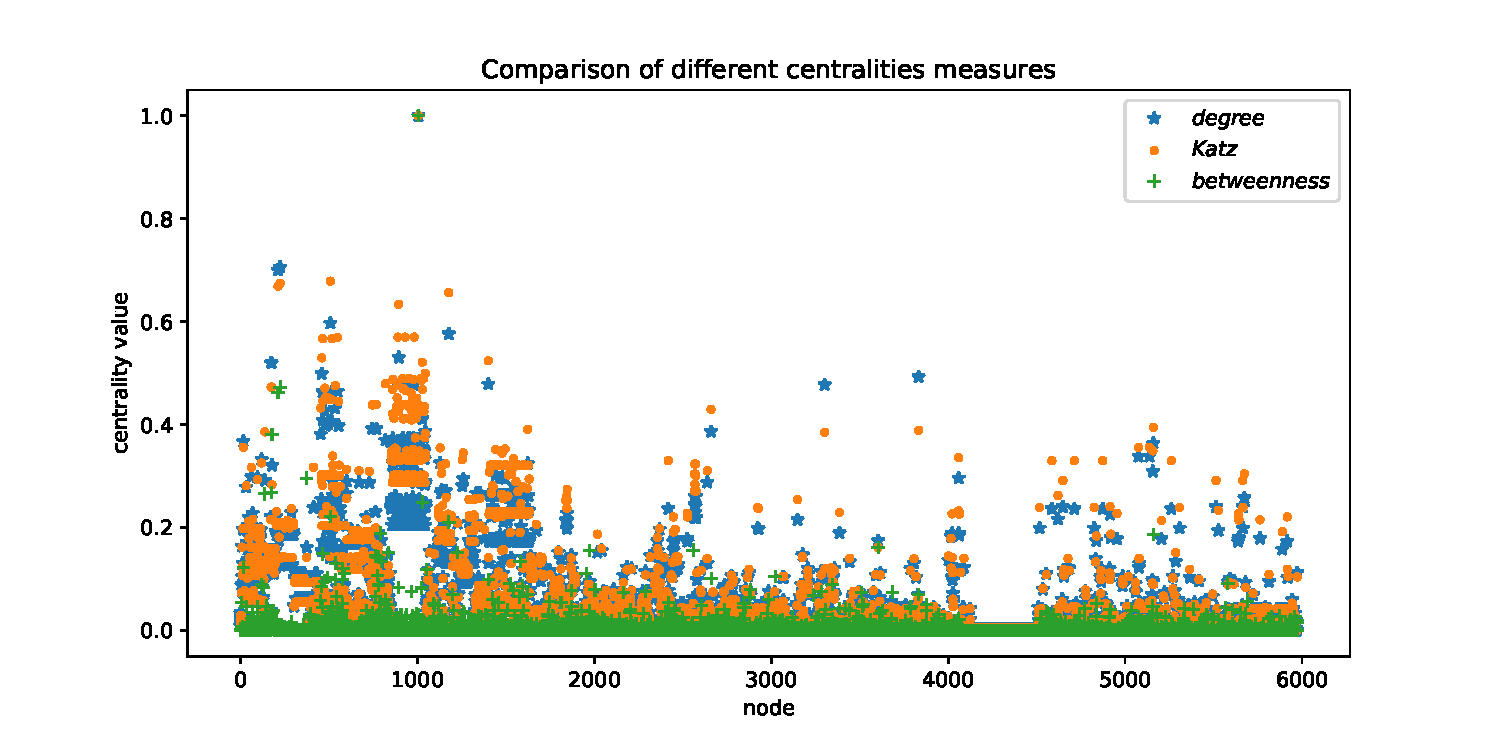
\includegraphics[width=.5\textwidth,clip, trim=0 0 0 0]{comparison}\label{fig:1_comparison_n}}
	\hfill
	\subfloat[sorted (increasing $C_{ka}$)]{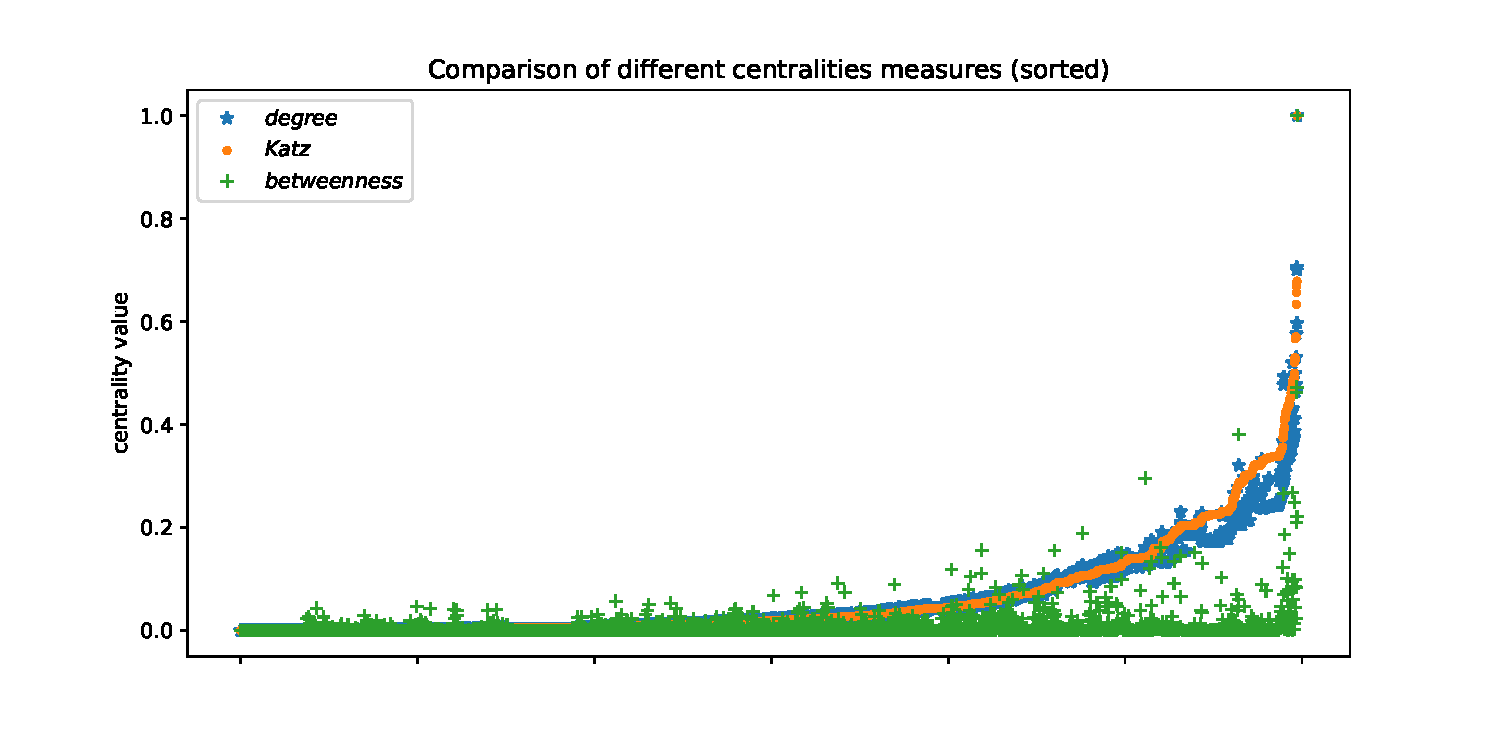
\includegraphics[width=.5\textwidth,clip, trim=0 0 0 0]{comparison_sort}\label{fig:1_comparison_sort}}
	\null\hfill
	\caption{Comparison of the different centralities indices}
	\label{fig:comparison}
\end{figure}

\pagebreak

\section{Epidemic processes over the graph}
%!TeX root = ../complex_net_report_senacheribbe.tex
\graphicspath{{../assignment2/figures/}}

\subsection{Introduction}

In this assignment, we simulated different epidemic processes on a real graph. The chosen network is a small snapshot of Facebook graph, obtained from users participating in an app (\cite{db_fb}). Each node represents a person, while the edges are friendship between people.\\
In \cref{fig:2_sparsity}, the sparsity of the adjacency matrix of the graph is reported. The blocky structure indicates the presence of different communities, ie part of the graph which are closely connected together.\\
% The numbering of the nodes is sorted such that nodes from the same community have adjacent numbers, yielding to these blocks around the diagonal.
It is interesting to study epidemic processes on social networks, because they are a good model for the spread of information across people.\\ Moreover, since our graph shows this community structure, we can try to see how the information spread inside a community and from one community to another.


\begin{figure} [!ht]
	\centering
	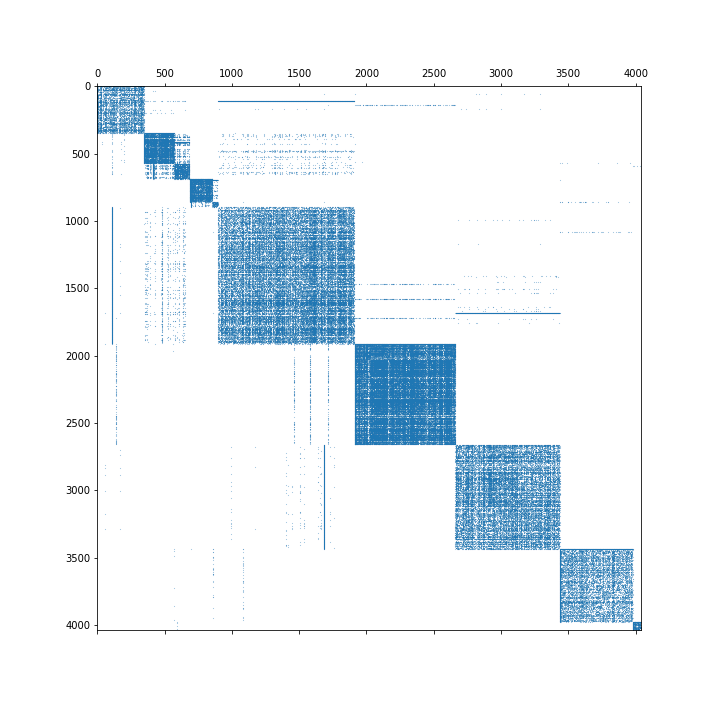
\includegraphics[width=.5\linewidth, clip, trim={2cm 2cm 2cm 2cm}]{sparsity}
	\caption{Sparsity of social network graph with  $n = 4039$ and $m = 88234$}
	\label{fig:2_sparsity}
\end{figure}


\subsection{Simple SI model}
The first model studied is a simple SI model: when a node is infected, it can infect with a probability $p$ each adjacent node. To implement this model, a FIFO queue is used to keep track of which infected node is to be processed and has to spread the infection to the neighbours. More details are reported in \cref{algo:2_simple}. The function  \textit{simple\_model} outputs:
\begin{itemize}
	\item $n\_infected$, a vector containing the number of infected nodes for each generation (generation is increased each time the infection spread to a neighbour node and it can represent the distance from the source node)
	\item $infected$, a vector that for each node associates 1 if was infected in the process, 0 otherwise. 
\end{itemize}

To test the model, we simulate an infection starting from node $\#2300$, which is in the middle of one community block.
We choose different values of $p$ (probability of spreading the infection) to test its effect on the process. Following a Monte Carlo approach, $1000$ simulations are run for each value of $p$ and the outputs are averaged. \\
The result of simulation are shown in \cref{fig:2_simple}, where we plot the fraction of infected nodes against the generations. $p=1$ is the degenerate case where all the neighbouring nodes get the infection and this is equivalent to a graph search (BFS).\\
From the graph we can notice that by increasing the generation, we have more nodes infected, since the algorithm is let run more and propagate for longer the infection. Moreover by increasing $p$, we have an higher probability to spread the infection, therefore an higher fraction of nodes gets infected.

\begin{figure} [!ht]
	\centering
	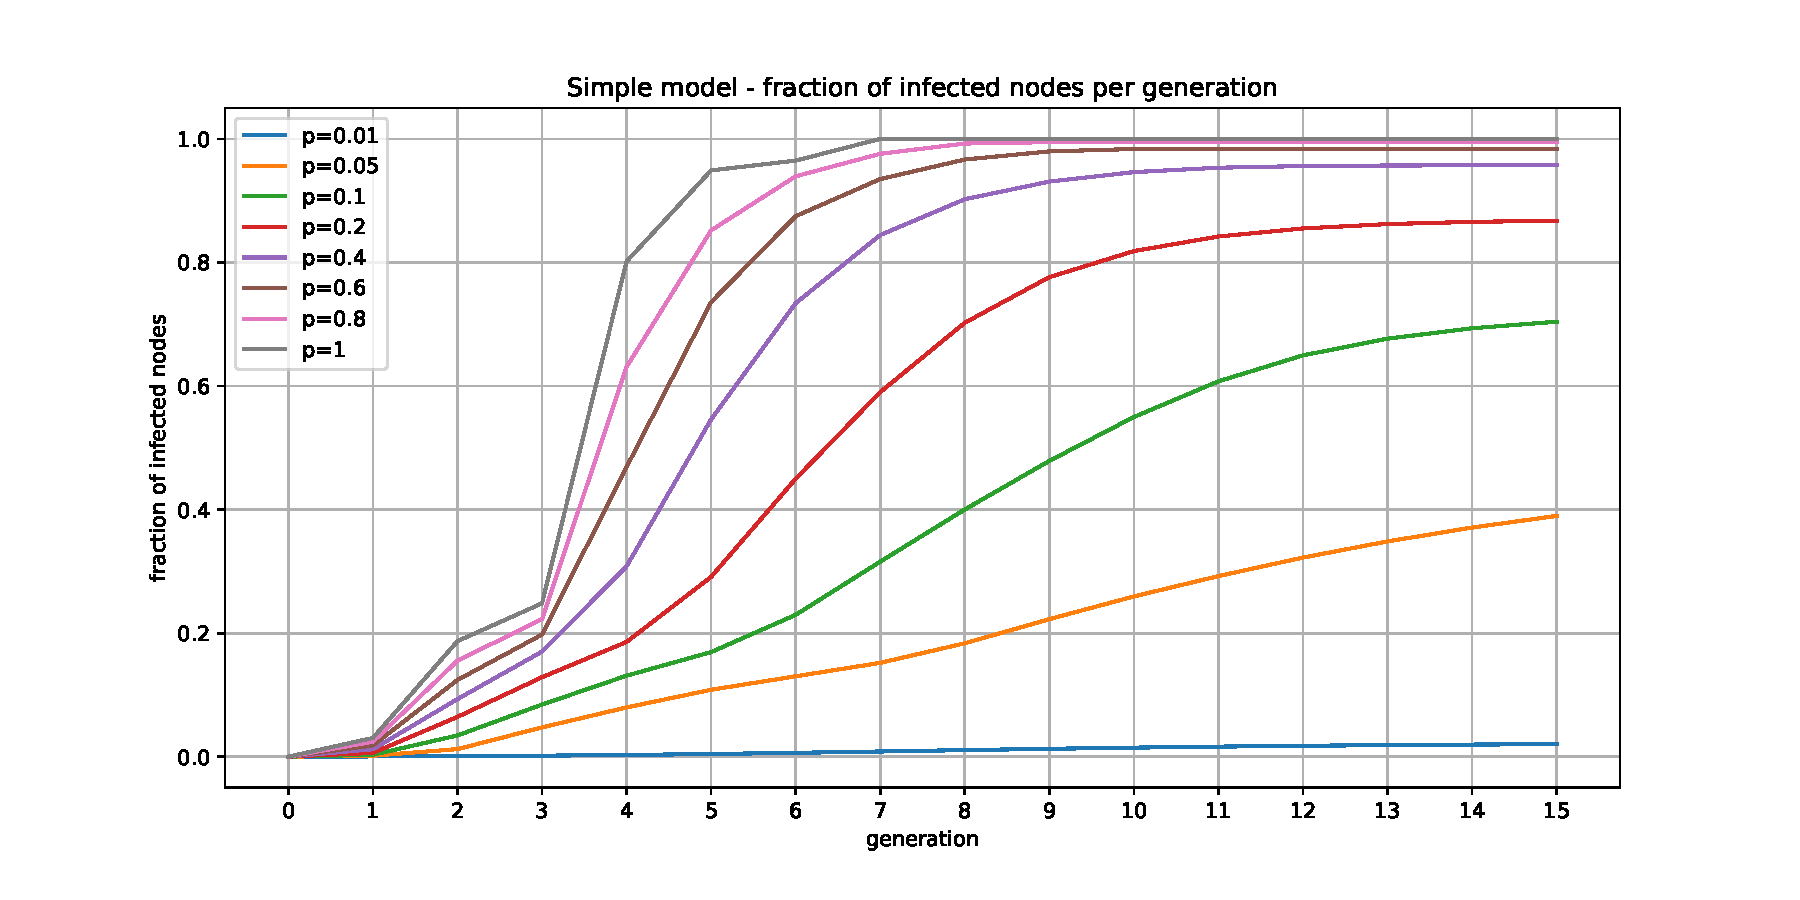
\includegraphics[width=.65\linewidth]{simple}
	\caption{Number of infected nodes per generation for the simple model algorithm}
	\label{fig:2_simple}
\end{figure}

In \cref{fig:2_probability} instead, the model has been run with $p=0.1$ for 8 generations, starting again from node $\#2300$ and averaging $1000$ simulations. The plot shows for each node the probability of it to be infected (1 means that in all $1000$ simulations it was infected, 0 if it was never infected). We can clearly notice the the information started in node $\#2300$ spreads easily in the community of the node itself and to the adjacent community of node $\#1500$ (probably because the two communities are well connected). The information struggles instead to be received from the other block communities.

\begin{figure} [!ht]
	\centering
	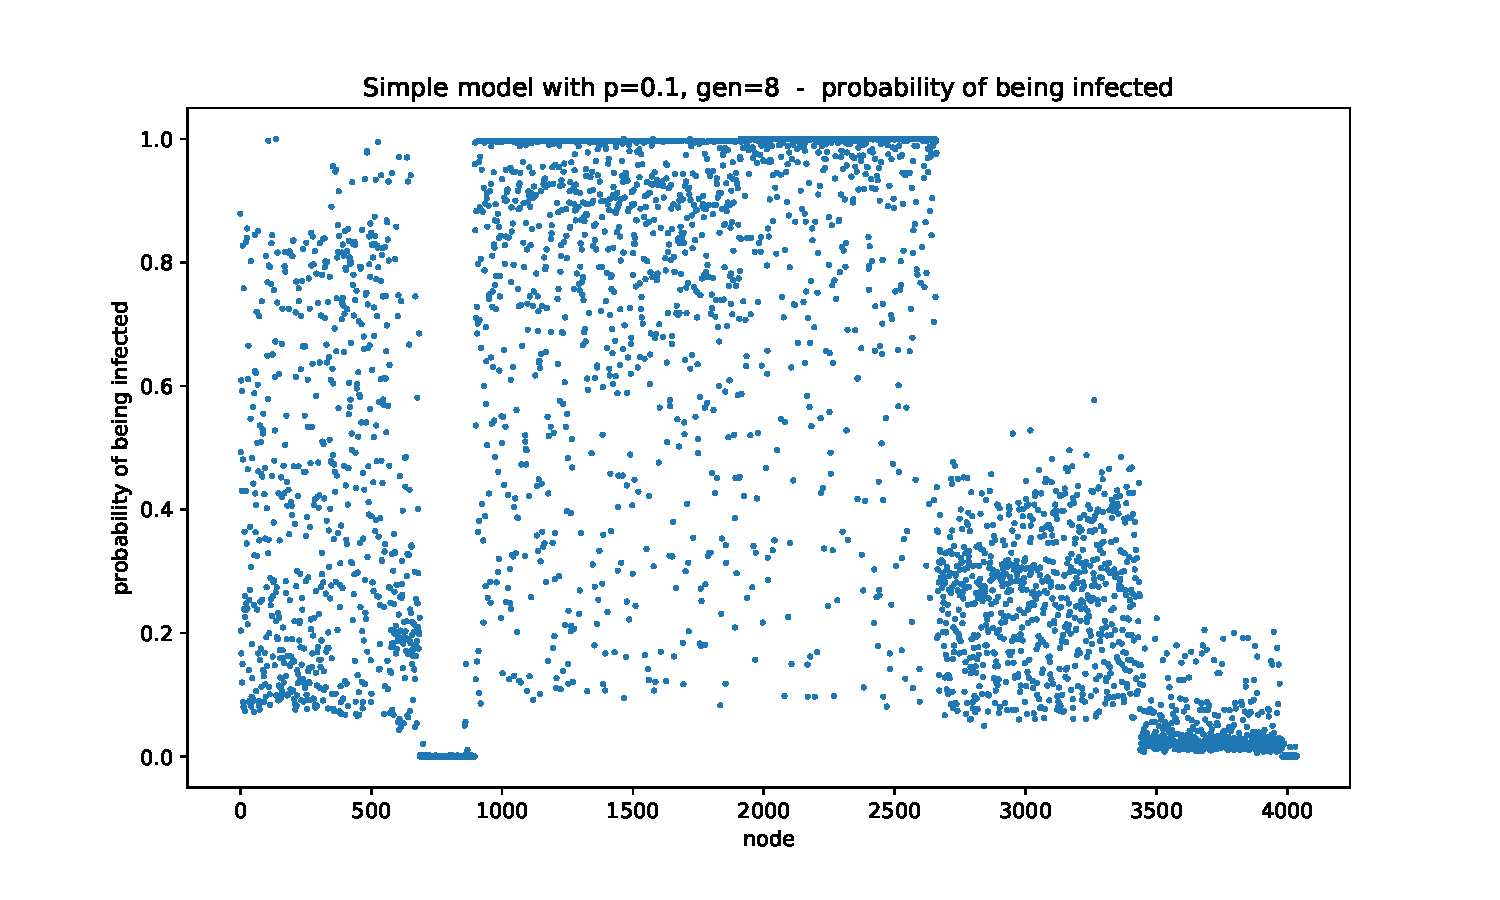
\includegraphics[width=.55\linewidth]{probability}
	\caption{Probability of being infected for the simple model algorithm}
	\label{fig:2_probability}
\end{figure}


\begin{algorithm}[!ht]
	\caption{Simple SI model}
	\label{algo:2_simple}
	\begin{algorithmic}[1]
		\Function{simple\_model}{$graph, p, max\_gen, starting$}
		
		\State $n\_infected \gets$ vector, size $max\_gen+1$, full of $0$
		\State $infected \gets$ vector, size $n$, full of $0$
		\State $queue \gets$ empty queue\\
		\Comment{$queue$ contains a tuple of 2 elements: node id and generation}
		\\
		
		\State enqueue $((starting, 0)) \to queue$
		\State $infected[starting] \gets 1$
		\State $n\_infected[0] \gets 1$	
		\\
		\While {$queue$ not empty and $g\le max\_gen$}
		\State dequeue $((v,g)) \gets queue$
		
		\For{$i \in $ neighbours of $v$}		
		\If{$infected[i]=0$ and $random()<p$} \Comment{$random() \sim Uniform[0,1]$}
		\State $infected[i] \gets 1$
		\State $n\_infected[g+1]+=1$				
		\State enqueue $((i, g+1)) \to queue$
		\EndIf
		\EndFor
		\EndWhile
		\\	
		\State \Return $cumsum(n\_infected)/n$ and $infected$
		\EndFunction
	\end{algorithmic}
\end{algorithm}

\subsection{Bootstrap percolation}\label{sec:2_boot}

As second epidemic process, we implemented the bootstrap percolation: a node gets infected if at least $r$ of its neighbours are infected. 
The pseudocode presented in \cref{algo:2_bootstrap} is very similar to \cref{algo:2_simple}, with the difference that $starting$ is now a vector of initial infected nodes and the addition of the vector $pressure$ which counts how many infected nodes are adjacent to the considered node. When the latter becomes $\ge r$ the considered node becomes infected itself and it's added in the queue.

The results of the simulations are shown in \cref{fig:2_bootstrap}, for different values of $r$. The starting points are 10 nodes inside the community of nodes from $\#2000$ to $\#2500$ (the same considered with the previous model). No Monte Carlo approach is needed, since once fixed the starting nodes, the spreading is deterministic. As we can notice from the picture, for the case $r=5$ the infection is not able to propagate, because too many adjacent nodes are required to get infected. Smaller values of $r$ makes easier to pass the infection. The case $r=1$ is a degenerate case, which is a simple graph search.

\begin{figure} [H]
	\centering
	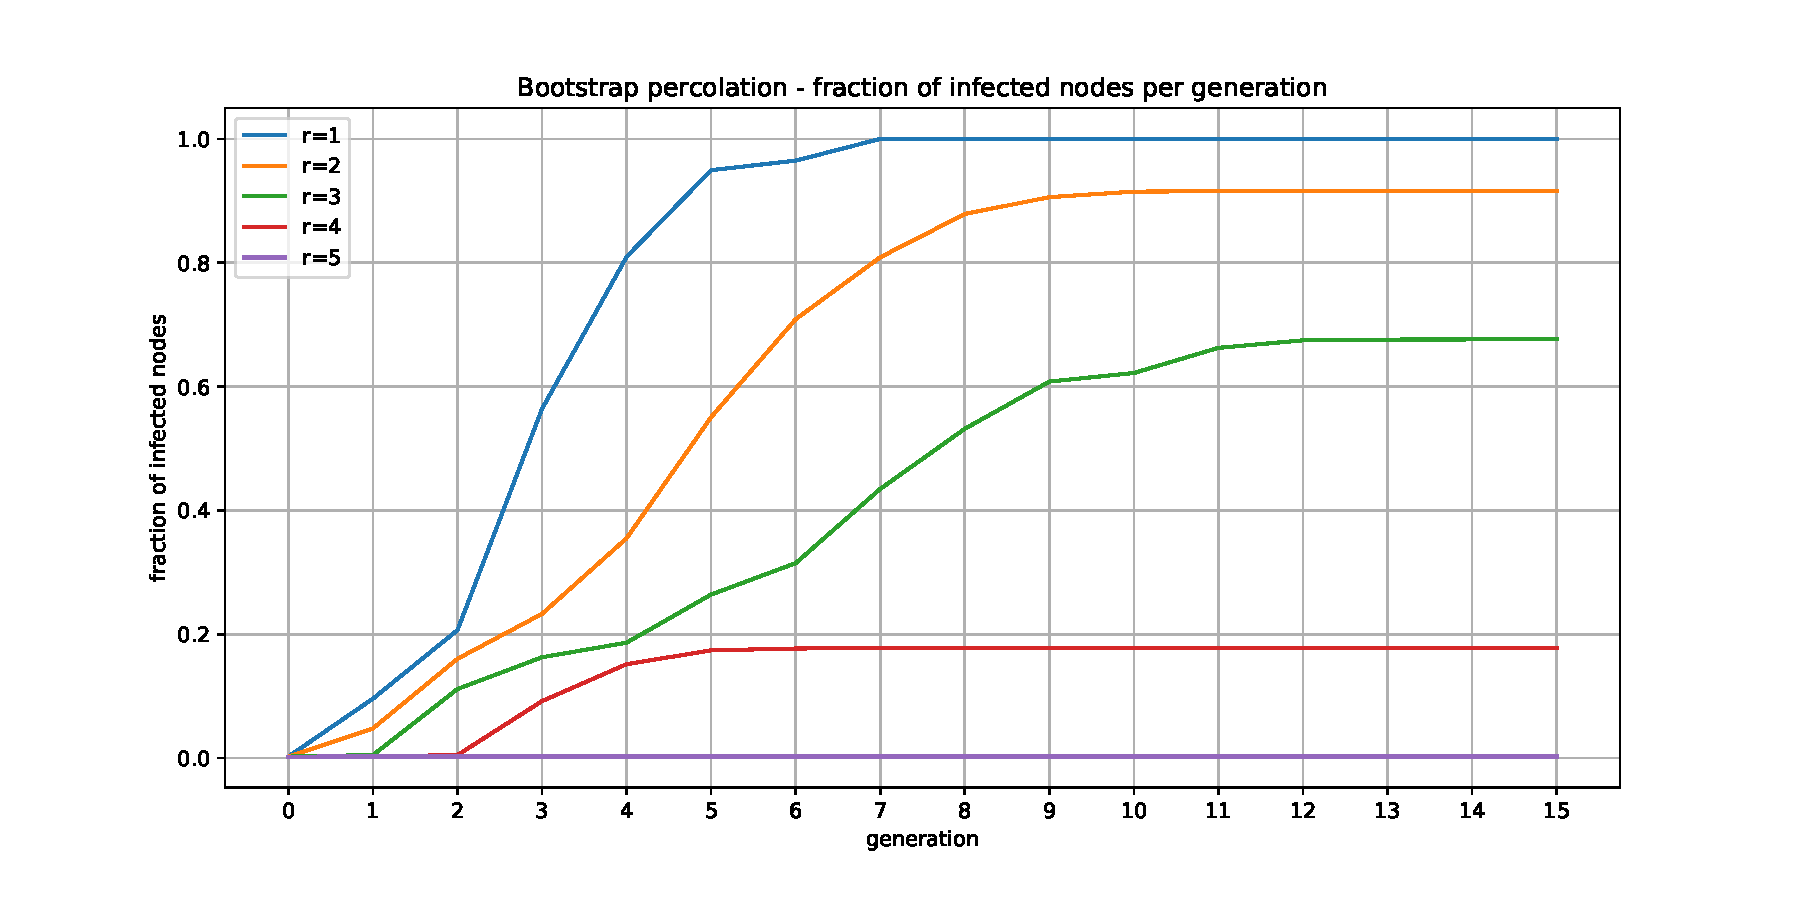
\includegraphics[width=.7\linewidth]{bootstrap}
	\caption{Number of infected nodes per generation for bootstrap percolation}
	\label{fig:2_bootstrap}
\end{figure}

\begin{algorithm}[H]
	\caption{Bootstrap percolation}
	\label{algo:2_bootstrap}
	\begin{algorithmic}[1]
		\Function{bootstrap\_percolation}{$graph, r, max\_gen, starting$}
		
		\State $n\_infected \gets$ vector, size $max\_gen+1$, full of $0$
		\State $infected \gets$ vector, size $n$, full of $0$
		\State $pressure \gets$ vector, size $n$, full of $0$
		\State $queue \gets$ empty queue\\
		\Comment{$queue$ contains a tuple of 2 elements: node id and generation}
		\\
		
		
		\State enqueue $((starting, 0)) \to queue$
		\State $infected[starting] \gets 1$
		\State $n\_infected[0] \gets length(starting)$	
		\\
		\While {$queue$ not empty and $g\le max\_gen$}
		\State dequeue $((v,g)) \gets queue$
		
		\For{$i \in $ neighbours of $v$}		
		\State $pressure[i] +=1$
		\If{$infected[i]=0$ and $pressure[i]\ge r$}
		\State $infected[i] \gets 1$
		\State $n\_infected[g+1]+=1$				
		\State enqueue $((i, g+1)) \to queue$
		\EndIf
		\EndFor
		\EndWhile
		\\	
		\State \Return $cumsum(n\_infected)/n$ and $infected$
		\EndFunction
	\end{algorithmic}
\end{algorithm}
\pagebreak

\subsection{Bootstrap percolation (stochastic version)}
Finally the bootstrap percolation presented in \cref{sec:2_boot} is modified to allow different values of $r$. Now instead of fixing it to a constant value, it is expressed as a vector that associates for each number of infected neighbours a probability to get the infection.\\ For example, the following mapping $r=[1 \to 0,\quad 2 \to 0.4,\quad 3 \to 1]$ means:
\begin{itemize}
	\item if a node has 1 infected neighbour $\rightarrow$ probability 0 of becoming infected
	\item if a node has 2 infected neighbours $\rightarrow$ probability 0.4 of becoming infected
	\item if a node has 3 or more infected neighbours $\rightarrow$ probability 1 of becoming infected
\end{itemize}
The sampling of the probability distribution is performed each time the number of adjacent infected neighbours changes. The algorithm to implement this version is exactly the same as \cref{algo:2_bootstrap}, with a small modification in the \textbf{If statement}.

Using the mapping above, we run $1000$ simulations and take the average. The starting points are the same 10 nodes between $\#2000$ and $\#2500$ considered before. The results are shown in \cref{fig:2_boot_stoc} and compared with a deterministic bootstrap with $r=2$ and $r=3$. As expected since our mapping is in the middle between $r=2$ and $r=3$ (we allow sometimes $r=2$ but always $r=3$), the curve representing the fraction of infected nodes is bounded by the two deterministic cases.

\begin{figure} [!ht]
	\centering
	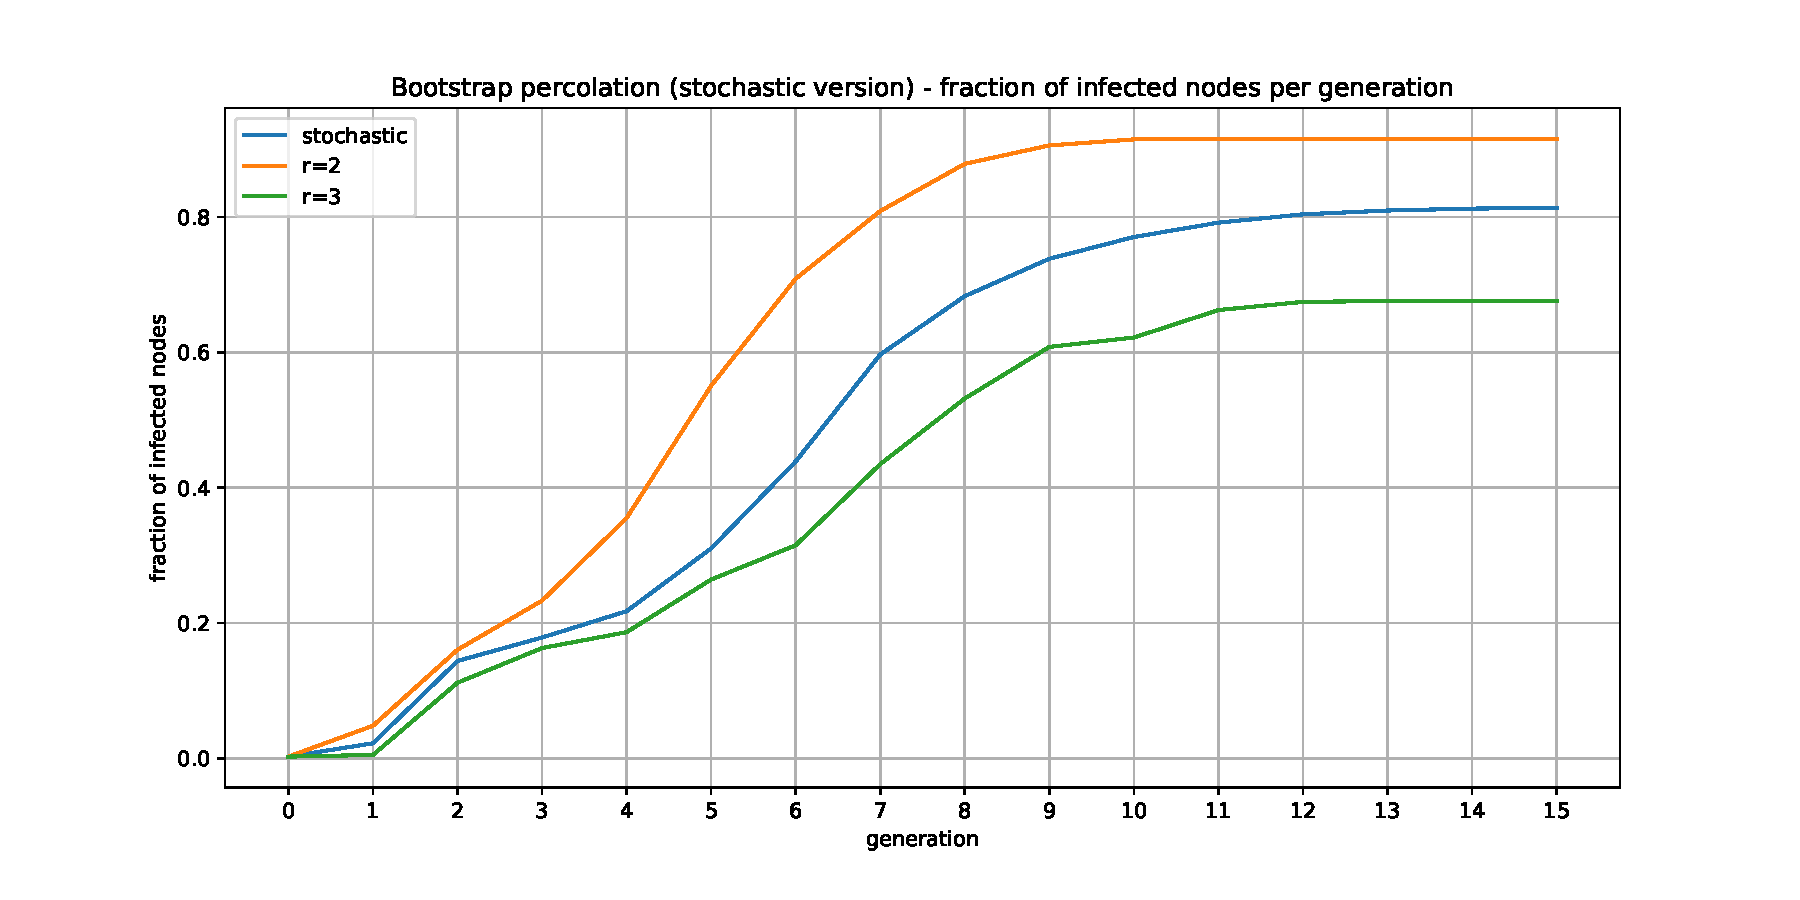
\includegraphics[width=.7\linewidth]{bootstrap_stoc}
	\caption{Number of infected nodes per generation for bootstrap percolation (stochastic version)}
	\label{fig:2_boot_stoc}
\end{figure}

\pagebreak

\section{Erdős–Rényi model}
%!TeX root = ../complex_net_report_senacheribbe.tex
\graphicspath{{../assignment3/figures/}}

\subsection{Introduction and graph generation}

The objective of this third assignment is to generate and test the properties of a $G(n,p)$ graph. To generate it, we propose the \cref{algo:3}. Essentially for each node $i$, we add an edge to $n\_edges$ random previous nodes, with $n\_edges \sim Binomial(i, p)$. To tackle the fact we only add edges to previous nodes, the sparse matrix is finally added to its transposed version, obtaining an undirected graph.\\
The time complexity of this algorithm is $O(n+m)$, in opposition to the naive approach of sampling a random variable for each possible entry of the matrix (would be $O(n^2)$, too much for large $n$).

\begin{algorithm}[!ht]
	\caption{Generate $G(n,p)$}
	\label{algo:3}
	\begin{algorithmic}[1]
		\Function{generate\_gnp}{$n,p$}
		\State $graph \gets$ sparse matrix, size $n\times n$
		\\
		\For{$i = 0 \to n$}		
		\State $n\_edges \gets Binomial(i, p)$ 
		\If{$n\_edges > 0$}
		\State $choices \gets $ pick $n\_edges$ \textbf{random} elements from $0...i$ (no repetitions)
		\State $graph[i, choices]=1$
		\EndIf
		\EndFor
		\\	
		\State \Return $graph+transpose(graph)$
		\EndFunction
	\end{algorithmic}
\end{algorithm}

The sparsity of a $G(1000,0.1)$ is reported in \cref{fig:3_sparsity}. The sparsity of the matrix is uniform (we don't have gaps or recognizable structures) and the number of edges ($m = 49721$) is compatible with the expected number of edges we know from theory
\begin{equation}
\mathbf{E} (m)=\frac{n(n-1)p}{2}=49950
\end{equation}

\begin{figure} [!ht]
	\centering
	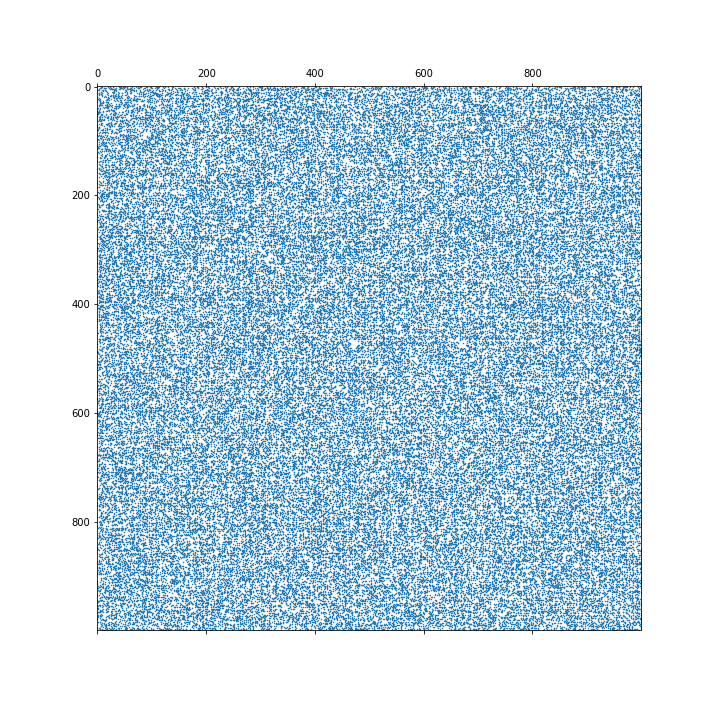
\includegraphics[width=.5\linewidth, clip, trim={2cm 2cm 2cm 2cm}]{sparsity}
	\caption{Sparsity of $G(n,p)$ with $n = 1000$ and $m = 49721$}
	\label{fig:3_sparsity}
\end{figure}


\subsection{Testing $G(n,p)$ properties}

To test the properties of the Erdős–Rényi model, we run several simulations varying both $n$ and $p(n)$. For each choice of the two parameters, $100$ simulations are performed and the results are averaged using a Monte Carlo approach.
The full set of results produced are reported in \cref{t:gnp}. Here we focus instead on the results for $n=100000$ (\cref{t:gnp_100000}), which is the largest $n$ we simulated (so more representative for an asymptotic analysis).
\pagebreak
\subsubsection{Distribution of node degree}
According to theory, the distribution of node degree should follow a binomial distribution (light tail). 
The minimum and maximum values of the node degree for all different $n$ and $p(n)$ are reported in \cref{t:gnp_100000}, while in \cref{fig:3_distr} the case $n = 100000$ and $p(n) = 2log(n)/n$ is shown.\\ As we can notice from the plot, the simulation fits perfectly a $Binomial(n-1, p)$.

\begin{figure} [!ht]
	\centering
	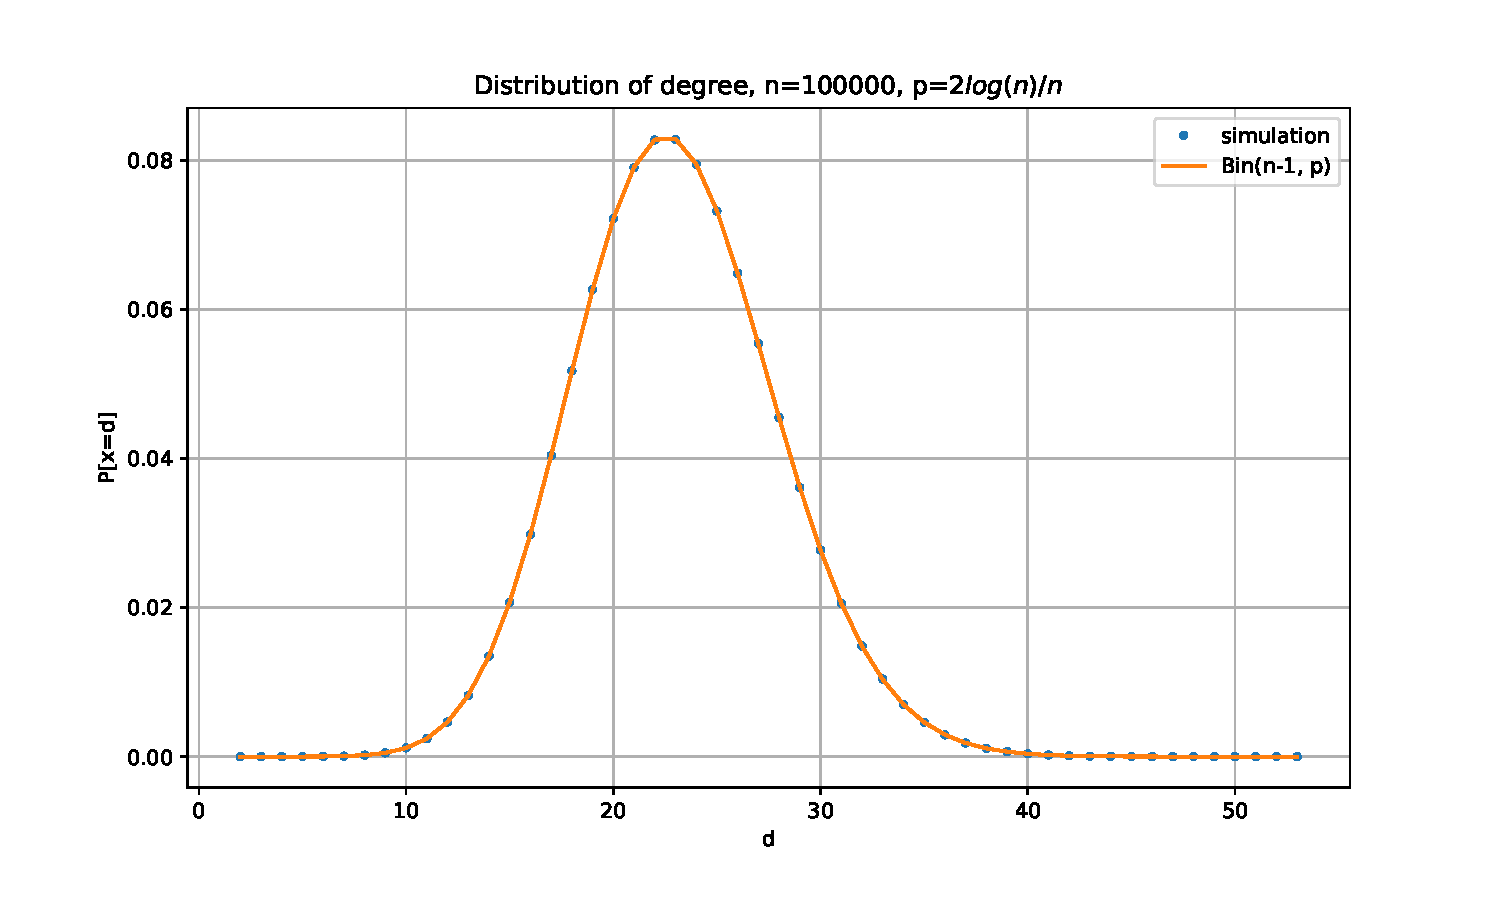
\includegraphics[width=.5\linewidth]{distribution}
	\caption{Distribution of degree $G(n,p)$ with $n = 100000$ and $p(n) = 2log(n)/n$}
	\label{fig:3_distr}
\end{figure}

\subsubsection{Diameter}
Calculating the exact diameter of a graph, ie the distance between the farthest nodes in the graph, is computationally expensive and not viable for large graphs like the one we are considering. We perform then an approximated calculation, which gives us a lower bound on the diameter. We sample randomly 20 nodes in the largest connected component and we compute the distance from them toward all the other nodes in the largest connected component.\\ The diameter is considered as the maximum distance found in this way. The results are reported in \cref{t:gnp_100000}. The first 2 rows should be excluded since the largest connected component is very small (we don't have a giant component). But from the third row, we can notice that $G(n,p)$ shows a small diameter ($\sim log(n)$), which decreases with increasing $p(n)$.

\subsubsection{Giant component}

The giant component is a connected component in which the number of nodes scales with $n$. To test its presence, we count the number of nodes in the largest connected component (\textit{1st cc}) and we consider it a giant component if it has at least $\frac{n}{10}$ nodes. In the column \textit{giant} of \cref{t:gnp_100000} we report the fraction of graphs that present this giant component (we run a Monte Carlo simulation with $100$ realisation for each $n$ and $p(n)$, 0 means none of the 100 graphs have this property, 1 all have it). \\
The transition from no giant to giant is abrupt between $0.9/n$ and $1.1/n$. As expected from theory, $1/n$ is a threshold function for the presence of the giant component. Moreover from the column \textit{2nd cc}, we can read the size of the second largest connected component. Again as expected from theory, when there is a giant component the 2nd connected component is a small component that scales at most with $log(n)$. The giant component is therefore unique.

\subsubsection{Connectivity}
Finally we analysed the connectivity of the graph. A graph is connected if there exists at least a path between any pair of nodes. Again from the table, we can notice that the graph is not connected up to the function $p(n)=0.9log(n)/n$ where we have a transition. $log(n)/n$ is a threshold function for the connectivity of the graph. We can also notice that approaching the threshold, the last nodes that remain outside the giant component and prevent the connectivity are isolated nodes (looking at \textit{2nd cc} we have it 1 for $0.9log(n)/n$ and $1.1 log(n)/n$).

\begin{table}[ht!]
	\centering
	\small
	\begin{tabular}{l|l|l|l|l|l|l|l}
		\toprule
		p(n) &  connected &  giant &  diameter &     1st cc &  2nd cc & deg\_min & deg\_max \\
		\midrule
		0.5/n &       0.00 &    0.0 &     12.55 &      25.90 &   22.47 &       0 &       8 \\
		0.9/n &       0.00 &    0.0 &     50.52 &     301.06 &  211.81 &       0 &       9 \\
		1.1/n &       0.00 &    1.0 &    160.08 &   17384.43 &  319.00 &       0 &      10 \\
		1.5/n &       0.00 &    1.0 &     52.59 &   58202.49 &   38.24 &       0 &      11 \\
		2/n &       0.00 &    1.0 &     31.90 &   79673.69 &   14.96 &       0 &      13 \\
		0.5 log(n)/n &       0.00 &    1.0 &     11.08 &   99678.32 &    2.02 &       0 &      22 \\
		0.9 log(n)/n &       0.03 &    1.0 &      7.60 &   99996.89 &    1.00 &       0 &      31 \\
		1.1 log(n)/n &       0.76 &    1.0 &      7.00 &   99999.74 &    1.00 &       0 &      38 \\
		1.5 log(n)/n &       1.00 &    1.0 &      6.00 &  100000.00 &     - &       1 &      44 \\
		2 log(n)/n &       1.00 &    1.0 &      5.00 &  100000.00 &     - &       2 &      54 \\
		0.01 &       1.00 &    1.0 &      3.00 &  100000.00 &     - &     153 &     490 \\
		\bottomrule
	\end{tabular}
\caption{Results from simulations of G(n,p), focus on $n=100000$}
\label{t:gnp_100000}
\end{table}

\begin{table}[ht!]
	\centering
	\small
	\begin{tabular}{l|l|l|l|l|l|l|l|l}
	\toprule
	n &          p(n) &  connected &  giant &  diameter &     1st cc &      2nd cc & deg\_min & deg\_max \\
	\midrule
	100 &         0.5/n &       0.00 &   0.05 &      3.89 &       5.90 &    4.310000 &       0 &       4 \\
	100 &         0.9/n &       0.00 &   0.71 &      8.07 &      14.88 &    7.990000 &       0 &       6 \\
	100 &         1.1/n &       0.00 &   0.92 &     11.76 &      27.47 &    9.270000 &       0 &       8 \\
	100 &         1.5/n &       0.00 &   1.00 &     15.03 &      53.39 &    7.190000 &       0 &       7 \\
	100 &           2/n &       0.00 &   1.00 &     13.68 &      78.19 &    3.710000 &       0 &       9 \\
	100 &  0.5 log(n)/n &       0.00 &   1.00 &     11.44 &      86.58 &    2.210000 &       0 &       9 \\
	100 &  0.9 log(n)/n &       0.21 &   1.00 &      6.69 &      98.46 &    1.050633 &       0 &      12 \\
	100 &  1.1 log(n)/n &       0.59 &   1.00 &      5.83 &      99.44 &    1.000000 &       0 &      14 \\
	100 &  1.5 log(n)/n &       0.85 &   1.00 &      4.43 &      99.84 &    1.000000 &       0 &      19 \\
	100 &    2 log(n)/n &       0.98 &   1.00 &      4.03 &      99.98 &    1.000000 &       0 &      23 \\
	100 &          0.01 &       0.00 &   0.82 &      9.34 &      19.72 &    8.430000 &       0 &       6 \\
	1000 &         0.5/n &       0.00 &   0.00 &      6.85 &      11.58 &    8.880000 &       0 &       5 \\
	1000 &         0.9/n &       0.00 &   0.09 &     19.13 &      56.58 &   28.490000 &       0 &       7 \\
	1000 &         1.1/n &       0.00 &   0.72 &     31.08 &     158.04 &   48.360000 &       0 &       8 \\
	1000 &         1.5/n &       0.00 &   1.00 &     30.76 &     579.34 &   14.720000 &       0 &       9 \\
	1000 &           2/n &       0.00 &   1.00 &     20.10 &     799.31 &    6.220000 &       0 &      10 \\
	1000 &  0.5 log(n)/n &       0.00 &   1.00 &     10.94 &     965.21 &    2.090000 &       0 &      14 \\
	1000 &  0.9 log(n)/n &       0.13 &   1.00 &      6.91 &     998.03 &    1.022989 &       0 &      18 \\
	1000 &  1.1 log(n)/n &       0.63 &   1.00 &      6.05 &     999.46 &    1.027027 &       0 &      21 \\
	1000 &  1.5 log(n)/n &       0.95 &   1.00 &      5.01 &     999.95 &    1.000000 &       0 &      29 \\
	1000 &    2 log(n)/n &       1.00 &   1.00 &      4.15 &    1000.00 &         - &       1 &      32 \\
	1000 &          0.01 &       0.96 &   1.00 &      5.04 &     999.96 &    1.000000 &       0 &      27 \\
	10000 &         0.5/n &       0.00 &   0.00 &      9.49 &      17.55 &   14.540000 &       0 &       7 \\
	10000 &         0.9/n &       0.00 &   0.00 &     30.81 &     134.35 &   89.460000 &       0 &       8 \\
	10000 &         1.1/n &       0.00 &   0.87 &     94.85 &    1676.05 &  169.850000 &       0 &       9 \\
	10000 &         1.5/n &       0.00 &   1.00 &     42.65 &    5825.63 &   24.420000 &       0 &      10 \\
	10000 &           2/n &       0.00 &   1.00 &     26.21 &    7967.78 &   10.300000 &       0 &      12 \\
	10000 &  0.5 log(n)/n &       0.00 &   1.00 &     10.90 &    9896.13 &    2.040000 &       0 &      18 \\
	10000 &  0.9 log(n)/n &       0.11 &   1.00 &      7.09 &    9997.51 &    1.000000 &       0 &      26 \\
	10000 &  1.1 log(n)/n &       0.71 &   1.00 &      6.18 &    9999.65 &    1.000000 &       0 &      30 \\
	10000 &  1.5 log(n)/n &       0.99 &   1.00 &      5.31 &    9999.99 &    1.000000 &       0 &      35 \\
	10000 &    2 log(n)/n &       1.00 &   1.00 &      5.00 &   10000.00 &         - &       2 &      42 \\
	10000 &          0.01 &       1.00 &   1.00 &      3.00 &   10000.00 &         - &      55 &     150 \\
	100000 &         0.5/n &       0.00 &   0.00 &     12.55 &      25.90 &   22.470000 &       0 &       8 \\
	100000 &         0.9/n &       0.00 &   0.00 &     50.52 &     301.06 &  211.810000 &       0 &       9 \\
	100000 &         1.1/n &       0.00 &   1.00 &    160.08 &   17384.43 &  319.000000 &       0 &      10 \\
	100000 &         1.5/n &       0.00 &   1.00 &     52.59 &   58202.49 &   38.240000 &       0 &      11 \\
	100000 &           2/n &       0.00 &   1.00 &     31.90 &   79673.69 &   14.960000 &       0 &      13 \\
	100000 &  0.5 log(n)/n &       0.00 &   1.00 &     11.08 &   99678.32 &    2.020000 &       0 &      22 \\
	100000 &  0.9 log(n)/n &       0.03 &   1.00 &      7.60 &   99996.89 &    1.000000 &       0 &      31 \\
	100000 &  1.1 log(n)/n &       0.76 &   1.00 &      7.00 &   99999.74 &    1.000000 &       0 &      38 \\
	100000 &  1.5 log(n)/n &       1.00 &   1.00 &      6.00 &  100000.00 &         - &       1 &      44 \\
	100000 &    2 log(n)/n &       1.00 &   1.00 &      5.00 &  100000.00 &         - &       2 &      54 \\
	100000 &          0.01 &       1.00 &   1.00 &      3.00 &  100000.00 &         - &     153 &     490 \\
	\bottomrule
\end{tabular}
\caption{Results from simulations of G(n,p)}
\label{t:gnp}
\end{table}
\pagebreak

\section{Barabási–Albert model}
%!TeX root = ../complex_net_report_senacheribbe.tex

\graphicspath{{../assignment4/figures/}}

\subsection{Introduction}
In this last assignment, we are required to implement the Barabási–Albert model and to test its properties. BA is a generative model, which means that the graph is defined through a process/algorithm and cannot be defined mathematically by associating a probability space (which can be done for instance for G(n,p)).
Simulations are therefore even more essential to study the properties of the model.

The main concept behind this model is the preferential attachment rule, according to which a new node that joins the network will be connected with higher probability to most popular nodes.
Indeed, we start from an initial graph and we add iteratively one node at a time and connect it to $m_{BA}$ nodes already in the graph (we didn't use the notation $m$ to avoid confusions with the number of edges). The probability $p_u$ for a new coming node to connect to a node $u$ in the graph is given by \cref{eq:pu_BA}
\begin{equation}
p_u = \frac{d_u^\gamma}{\sum_{v \in V}{d_v^\gamma}}\label{eq:pu_BA}
\end{equation}
where $d_u$ is the current degree of the node $u$ and $\gamma$ is the exponent that defines the proportion between $p_u$ and $d_u$.

\subsection{Algorithms}
We now present two different algorithms to create a BA graph. The first approach adopted, which is presented in \cref{algo:ba_opt}, is able to generate very efficiently a BA graph for the case $p_u \propto d_u$. It's employing essentially an additional vector ($urn$) which is constructed so that the number of times each node $i$ of the graph appears in the vector is equal to the $deg(i)$. Picking a random element from $urn$ corresponds then to sampling the discrete distribution described in \cref{eq:pu_BA} with $\gamma=1$.

The second approach (\cref{algo:ba}) instead computes the distribution each time and samples it, instead of employing an auxiliary vector. This method is more computationally expensive, but it's the only viable for the case $p_u \not\propto d_u$. To further optimize it, the cumulative distribution to perform the sampling from is not computed entirely, but just for the portion needed. Notice indeed in the function \textit{random\_choice} described in \cref{algo:ba_r_c} the use of $sum\_p_u=\sum_{u} p_u$, so that we don't have to loop over all nodes in $p_u$ to compute the sum and the \textit{while} in line 14 that stops as soon as a new value is picked.\\
With this optimisation, especially for the case $p_u \propto d_u^{\gamma}$ with $\gamma>1$, the sampling can be computed very fast, because the initial nodes are big hubs, usually chosen for the new edges. The computation of the distribution is therefore stopped after few iterations.
We reduced in this way the average case complexity, while the worst case one remains still the same.
 
\subsection{Results}
In \cref{fig:sparsity4}, we report the sparsity of the adjacency matrix of a Barabási–Albert graph generated with $n=1000$ and $m_{BA}=3$. As expected, older nodes (first rows and columns) have more connections (more dense points), since they had more chances to be chosen from new nodes.

\begin{figure} [!ht]
	\centering
	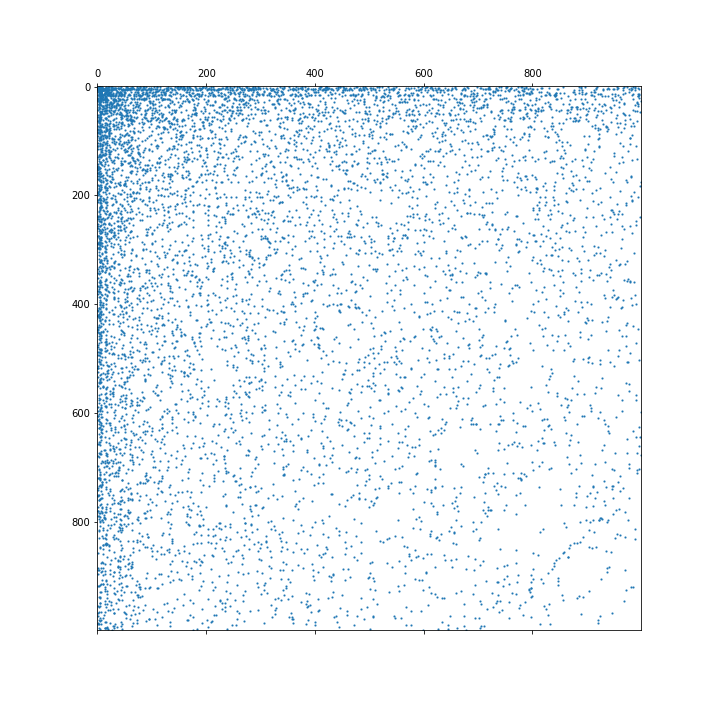
\includegraphics[width=.6\linewidth, clip, trim={2cm 2cm 2cm 2cm}]{sparsity}
	\caption{Sparsity of Barabási–Albert graph with $n=1000$, $m_{BA}=3$ and $m=3990$ (number of edges)}
	\label{fig:sparsity4}
\end{figure}
\pagebreak
The model was then run with $n=100000$ and $m_{BA}=3$, for the case $p_u \propto d_u$, $p_u \propto \sqrt{d_u}$ and $p_u \propto d_u^{1.5}$ (\cref{algo:ba_opt} was used for the case  $p_u \propto d_u$, while \cref{algo:ba} for the other two). For each of these functions of the degree, 100 graphs were generated. Following a Monte Carlo approach, the results shown in \cref{t:res4} and \cref{fig:deg4_gamma1,fig:deg4_gammacomp} are an average on those realisations.\\

\begin{table}[ht!]
	\centering
	\begin{tabular}{ |c|c|c|c| } 
		\hline
		gamma $\gamma$ & diameter &  clustering & max degree\\
		\hline
		1 & 7.54 & 0.000886 & 1540\\
		0.5 & 8.52 & 0.000120 & 110\\
		1.5 & 3.50 & 0.845655 & 97321\\
		\hline
	\end{tabular}
	\caption{Results for BA, $n=100000$,  $m_{BA}=3$, average from $100$ graphs for each $\gamma$}
	\label{t:res4}
\end{table}
\begin{figure} [!ht]
	\centering
	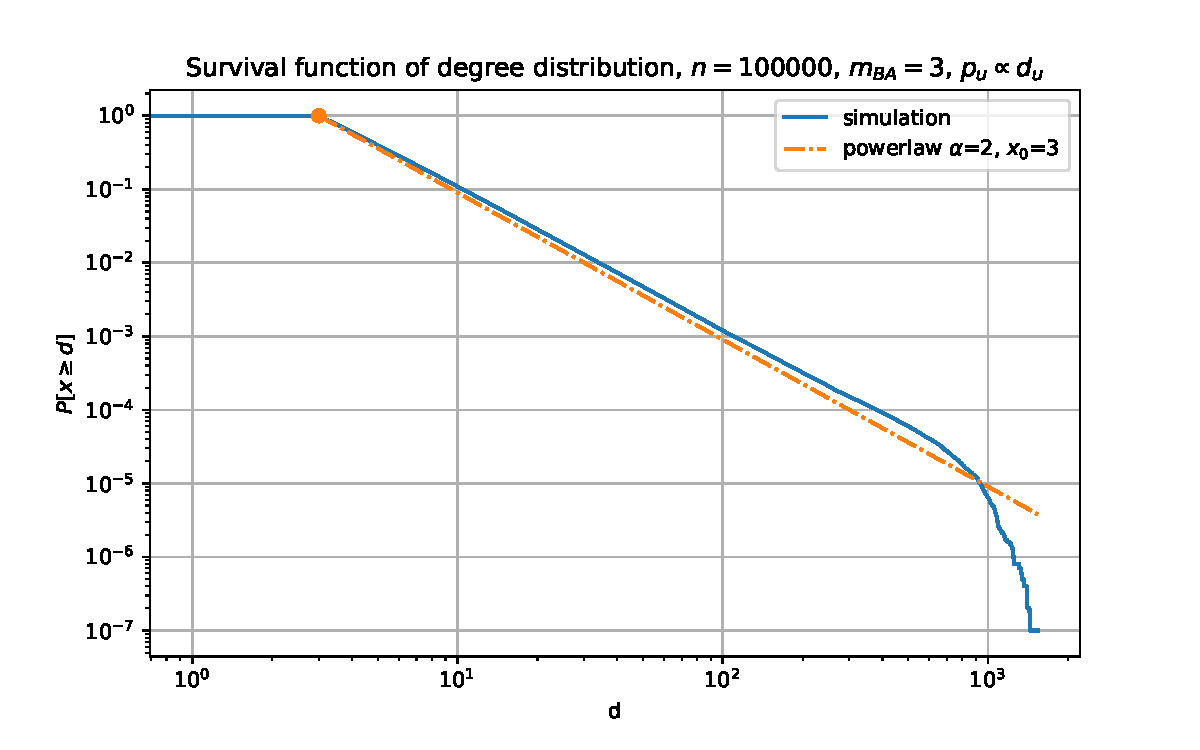
\includegraphics[width=.5\linewidth]{deg_gamma1}
	\caption{Survival function of degree distribution, BA with $n=100000$,  $m_{BA}=3$, $\gamma=1$}
	\label{fig:deg4_gamma1}
\end{figure}

The clustering coefficient is computed approximately by taking at random 50000 nodes, and for each node picking 2 random neighbours (without repetition) and check if they are connected. The clustering coefficient is then simply the number of connected triples found divided by the number of trials (50000 in our case).
The approximated diameter is found instead by computing, starting from 20 random nodes (without repetition), the maximum of distances toward all the other nodes.

\pagebreak

The result we obtain for $\gamma=1$ are compatible with the theory for BA. Indeed we get a powerlaw for the degree distribution with coefficient 3 for the pdf
\begin{equation}
P[d_u=k] \propto \frac{1}{k^3}
\end{equation}
which correspond to a coefficient of 2 for the cumulative as plotted in \cref{fig:deg4_gamma1}. \\As expected, the average diameter is small $diam=7.54$. Also the clustering coefficient is very small, $C= 0.000886$.\\

Different results are obtained for the case in which $\gamma \neq 1$. In \cref{fig:deg4_gammacomp} we compare the distribution of degree for different $\gamma$. For the case $p_u \propto \sqrt{d_u}$ the distribution decreases faster than the previous case and it's more concentrated for lower degrees.\\
The clustering is lower and the diameter is larger with respect to the simulations for $\gamma=1$. This is producing a weaker preferential attachment.\\
For $p_u \propto d_u^{1.5}$, on the other hand, the distribution indicates the presence of very high degree nodes. Notice from \cref{t:res4} that the maximum degree is 3 order of magnitude larger than the $\gamma=1$ case. 
What happens here is that few nodes start to become larger and larger and this trend is accelerated by the superlinear relation of $p_u$ and $d_u$. This is a stronger version of the preferential attachment.
Since the presence of these big hubs, the diameter is reduced and the clustering is increased.

\begin{figure} [!ht]
	\centering
	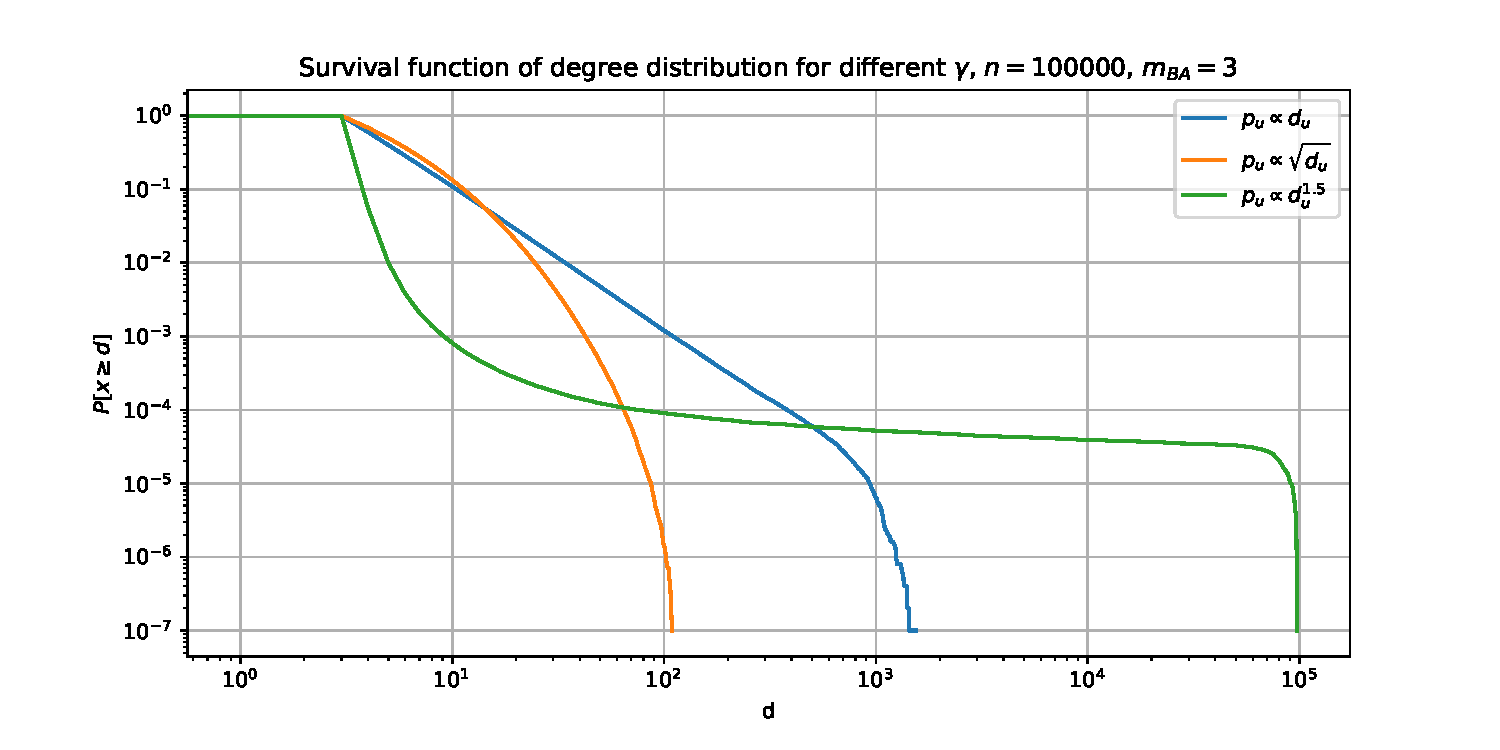
\includegraphics[width=.55\linewidth]{deg_gammacomp}
	\caption{Comparison of degree distributions for different values of gamma}
	\label{fig:deg4_gammacomp}
\end{figure}

\pagebreak
 
\begin{algorithm}
	\caption{Optimized algorithm to generate BA for the case $p_u \propto d_u$}
	\label{algo:ba_opt}
\begin{algorithmic}[1]
	\Function{generateBA}{$n, m_{BA}$}
		
		\State $graph \gets$ sparse matrix, size $n\times n$
		\State $urn \gets$ vector, size $2 n m_{BA}$
		\\
		\State $u \gets 1$
		\While {$u < m_{BA}+1$} \Comment{generate a complete graph of $m_{BA}+1$ nodes}
		\State $graph[u][0...u] \gets 1$
		
		\State $urn[len(urn) ... len(urn)+m_{BA}] \gets u$
		
		\State $u \gets u+1$
		\EndWhile
		\\
		\\
		\While {$u < n$} \Comment{add a new node at each iteration}
		\\
			\State $choices \gets $ pick $m$ \textbf{random} elements from $ urn $ (no repetitions)
			\\
			\State $graph[u][choices] \gets 1$ \Comment{connect node $u$ to all nodes in $choices$}
			\\
			\State $urn[len(urn) ... len(urn)+m_{BA}] \gets u$
			\State $urn[len(urn) ... len(urn)+m_{BA}] \gets choices$

		
		\State $u \gets u+1$
		\EndWhile
		\\	
		\State \Return $graph+transpose(graph)$
		\EndFunction
\end{algorithmic}
\end{algorithm}

\begin{algorithm}
	\caption{Generate BA, recomputing each time the distribution}
	\label{algo:ba}
	\begin{algorithmic}[1]
		\Function{generateBA}{$n, m_{BA}, f(x)=x^\gamma$}
		
		\State $graph \gets$ sparse matrix, size $n\times n$
		\State $d_u \gets$ vector, size $n$, full of $m$ \Comment{$d_u$ is the degree of each node, initially set to $m_{BA}$}
		\State $p_u \gets$ vector, size $n$, full of $f(m_{BA})$
		\\ \Comment{$p_u$ is the probability \underline{not normalized} to pick a node}
		\\
		\State $sum\_p_u \gets 0$  \Comment{$sum\_p_u$ is the $\sum_{u}{p_u}$}
		
		\\
		\State $u \gets 1$
		\While {$u < m_{BA}+1$} \Comment{generate a complete graph of $m_{BA}+1$ nodes}
		\State $graph[u][0...u] \gets 1$
		
		\State $u \gets u+1$
		\EndWhile
		\\
		\State $sum\_p_u \gets (m_{BA}+1)*f(m_{BA})$ 
		\\\Comment{update the sum: added $m_{BA}$ nodes with degree $m_{BA}$}
		\\
		\While {$u < n$} \Comment{add a new node at each iteration}
		\\
		\State $choices \gets random\_choice(size=m_{BA},p=p_u[0...u], sum\_p=sum\_p_u)$
		\\
		\State $graph[u][choices] \gets 1$ \Comment{connect node $u$ to all nodes in $choices$}
		\\
		\State $sum\_p_u-=p_u[choices]$	\Comment{update the $d_u$, $p_u$ and $sum\_p_u$ after the addition}
		\State $d_u[choices]+=1$
		\State $p_u[choices]=f(d_u[choices])$
		\State $sum\_p_u +=p_u[choices]$
		\\
		
		\State $u \gets u+1$
		\EndWhile
		\\	
		\State \Return $graph+transpose(graph)$
		\EndFunction
	\end{algorithmic}

\end{algorithm}

\begin{algorithm}
	\caption{Function $random\_choice$ to perform sampling from a discrete distribution}
	\label{algo:ba_r_c}
	\begin{algorithmic}[1]
		\Function{random\_choice}{$size,p, sum\_p$}
		\State $cdf \gets $ vector, size $length(p)$
		\State $choices \gets $ vector, size $size$
		
		\State  $cdf[0]=p[0]$
		\\
		\State $i \gets 0$
		\While{$i<size$} \Comment{loop on the number of choices to make}
		\State $r \gets random()*sum\_p_u$ \Comment{$random()$ returns a $Uniform[0,1]$}
		\\
		\If{$r<cdf[j]$}\Comment{if $r$ was in the part of $ cdf $ already computed}
		\\
		\State $new \gets $ binary search in $cdf[0...j+1]$, such that $cdf[new]\leq r < cdf[new+1]$
		\Else
		\While{$cdf[j]<r$} \Comment{continue to compute the $cdf$}
		\State $j+=1$
		\State $cdf[j]\gets cdf[j-1] + p[j]$
		\EndWhile
		\\
		\State $new \gets j$ \Comment{since the while stopped, $j$ is inside the block}
		\EndIf
		\\
		\If{$new$ is not already in $choices$}
		\State $choices[i] \gets new$
		\State $i+=1$
		\EndIf
		\EndWhile
		\\
		\State \Return $choices$
		\EndFunction
	\end{algorithmic}
	
\end{algorithm}




\newpage
\printbibliography

\end{document}